\chapter{Methodology}
\section{Overview of the Workflow}
In order to overcome the possible drawbacks of standalone techniques, the analysis uses a hybrid modeling framework that combines the advantages of machine learning and linear time series analysis. This approach expands upon the research of \cite{zhang2003hybrid}, who showed that forecast accuracy in complex time series can be greatly increased by mixing linear and non-linear models. A structured pipeline is used in the workflow, which is depicted in Figure \ref{fig:Flow chart}. Its goal is to systematically capture both linear and non-linear dependencies while preventing overfitting employing a Validation set.
\begin{figure}[H]
    \centering
    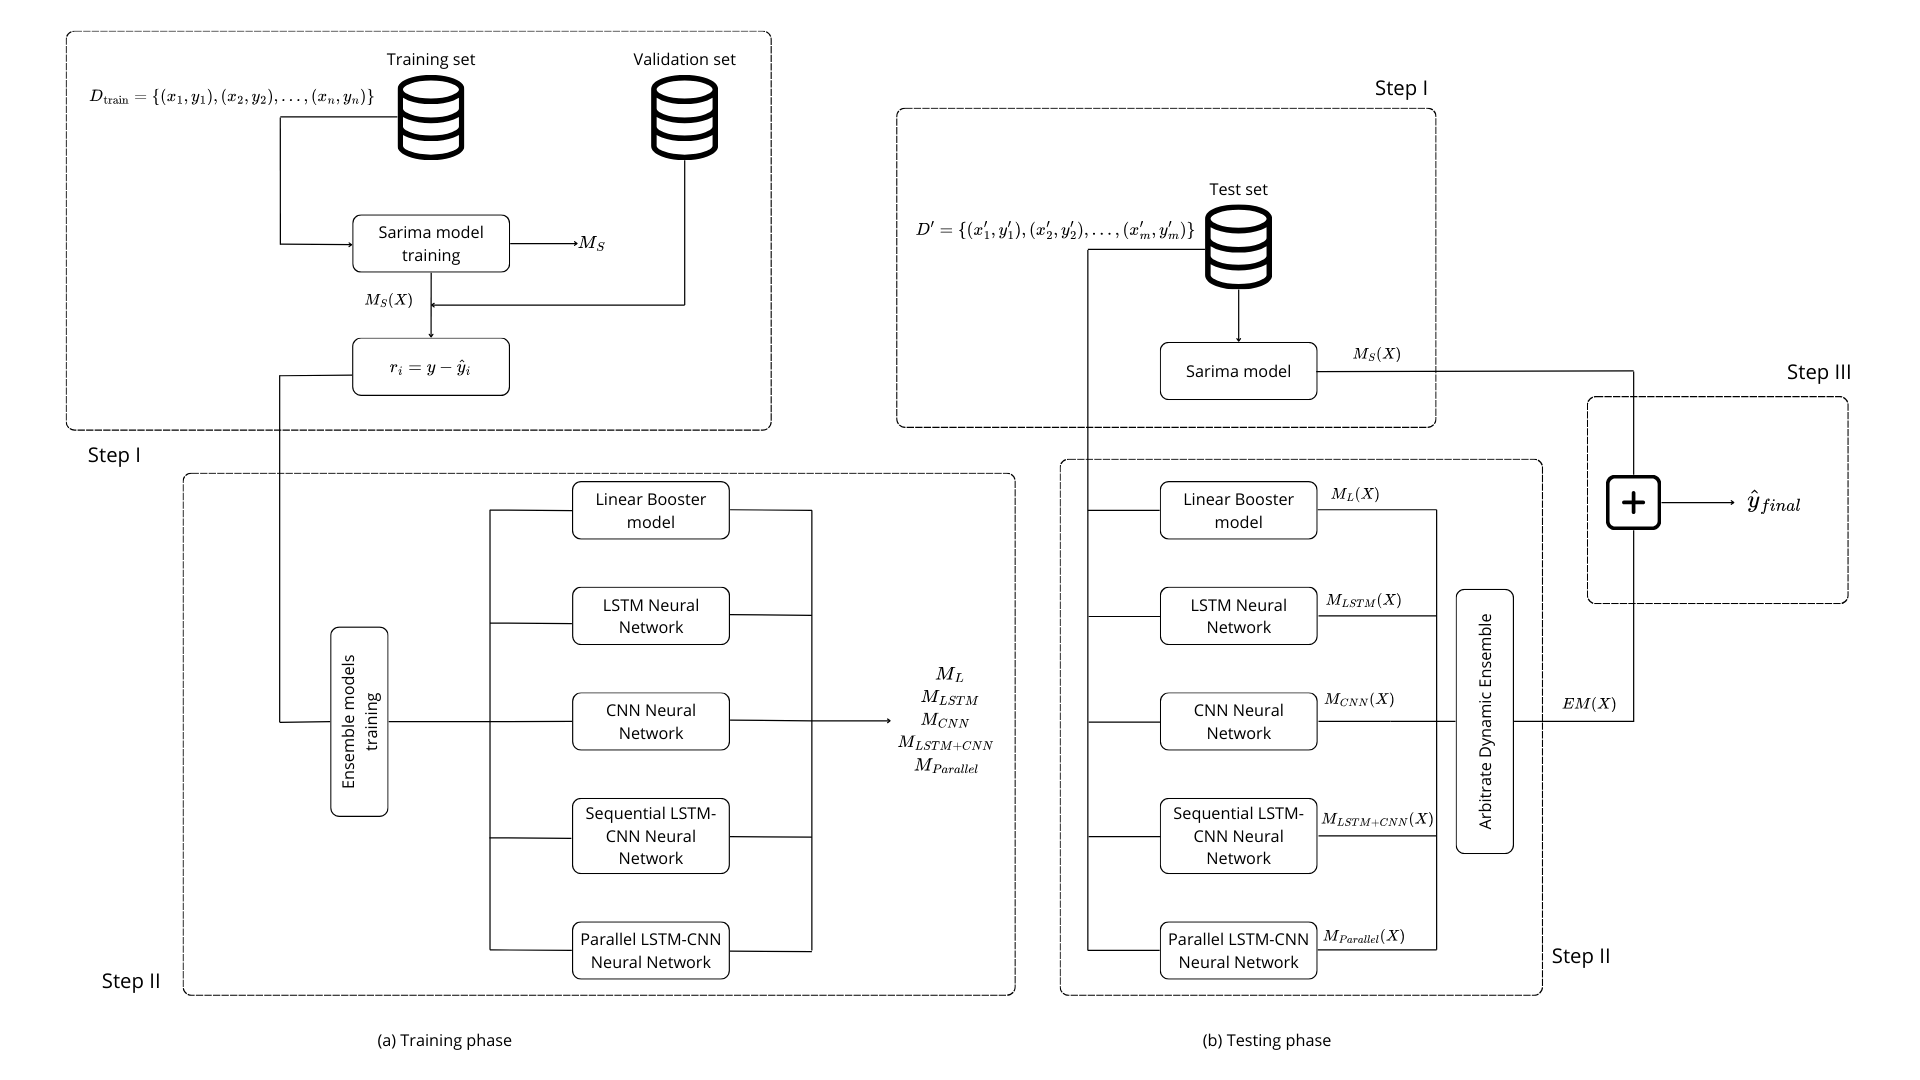
\includegraphics[width=0.90\textwidth]{Machine_learning_thesis/Images/Flow_chart.png}
    \caption{Flow chart of the analysis.} 
    \label{fig:Flow chart}
\end{figure}

\subsubsection{Training phase}
\textbf{Step I}

Seasonal Autoregressive Integrated Moving Average (SARIMA) modeling is the first step in the process. It is a proven technique for identifying linear dependencies in time series data \cite{Hyndman2018}. Because of its parameter structure $(p, d, q)(P, D, Q)_s$, SARIMA is especially good at modeling trends and seasonal patterns in the training data. Following training, predictions are made using the validation set, which includes out-of-sample data not used for fitting the model. The residuals are then computed as follows:
\[
\epsilon_t = y_{\text{val},t} - \hat{y}_{\text{val},t}
\]
Where:
\begin{itemize}
    \item \(\epsilon_t\) represents the residual at time
    \item \(y_{\text{val},t}\) is the actual observation
    \item \(\hat{y}_{\text{val},t}\) is the SARIMA prediction
\end{itemize}

These residuals contain valuable information about patterns that the linear model failed to capture, including potential non-linear relationships, abrupt regime changes, or complex interactions between variables \cite{Khashei2011}.

\textbf{Step II}

To model the remaining non-linear dependencies, a collection of machine learning and deep learning models is trained using these residuals $\epsilon_t$.


\subsubsection{Testing Phase and Performance Validation}
The testing phase evaluates the hybrid model’s generalizability on entirely  unseen data through a structured three-step workflow (Figure \ref{fig:Flow chart}), objectively quantifying its statistical significance and predictive accuracy. In the 

\textbf{Step I}

The trained SARIMA model generates the baseline forecasts \(\hat{y}_{\text{SARIMA,test}}\) on the test set, capturing linear dependencies (trends, seasonality, and autocorrelation) identified during training.

\textbf{Step II}

The residual series $\epsilon_{test} = y_{test} - \hat{y}_{SARIMA,test}$ is fed into the pre-trained ensemble of machine learning and deep learning models. These models predict the non-linear residuals $\hat{\epsilon}_{ML,test}$, leveraging their capacity to identify complex patterns in the SARIMA’s unexplained variance \cite{Goodfellow2016}. Then the Arbitrated Dynamic Ensemble optimally combines these forecasts by assigning time-varying weights according to each model's most recent accuracy.

\textbf{Step III}

Finally, predictions are aggregated additively:
\[
\hat{y}_t = \text{SARIMA}(p, d, q)(P, D, Q)_s + \hat{\epsilon}_{\text{ML}}
\]

\section{Data Preparation and Preprocessing} 
To implement the previously described procedure two distinct univariate time series datasets were selected: the S\&P 500 close price (spanning from 2000 to 2025) and the EUR/USD exchange rate (from 2003 to 2025). These data sets were selected to consider different characteristics that are commonly found in finance time series. The close price of the S\&P 500, which captures the market valuation of the top 500 publicly traded companies in the US, displays a distinct increasing trend alongside volatility clustering, which are indicative of the equity indexes' long-term growth and recurring market shocks \cite{Cont2001}. The EUR/USD exchange rate, on the other hand, is a typical example of currency markets where where trends are less dominant and seasonality is often subtle \cite{Cellini2011}. The datasets were retrieved using the \texttt{yfinance} API,  a reliable and widely adopted tool for financial time series extraction. Both series shows daily trading data with no missing observations, so there was no need for inputation.

\subsubsection{SARIMA preprocessing:}

To ensure stationarity, which is a crucial prerequisite for SARIMA modeling, the closing prices are transformed into logarithmic returns using the formula:
\[
r_t = \ln\left(\frac{P_{t-1}}{P_t}\right)
\]
where: 
\begin{itemize}
    \item $r_t$ represents the log return at time t
    \item $P_t$ is the closing price at time t.
\end{itemize}
This transformation achieves two key objectives: first, it stabilizes variance and eliminates multiplicative trends that are inherent in financial time series and second log returns exhibit time-additivity, meaning that the the cumulative return over n periods equals to the sum of individual log returns:
\[
r_{t:t+n} = \sum_{i=1}^{n} r_{t+i}.
\]
The stationarity is then verified using the Augmented Dickey-Fuller (ADF) test,which assesses the null hypothesis of a unit root (non-stationarity) in the series. The ADF test on the log returns for both datasets produced p-values less than 0.01, thus allowing the null hypothesis to be rejected, ensuring that the transformed time series is stationary, as evident by the absence of visible trends in the log return series. (Figure \ref{fig:Log returns}).
\begin{figure}[H]
    \centering
    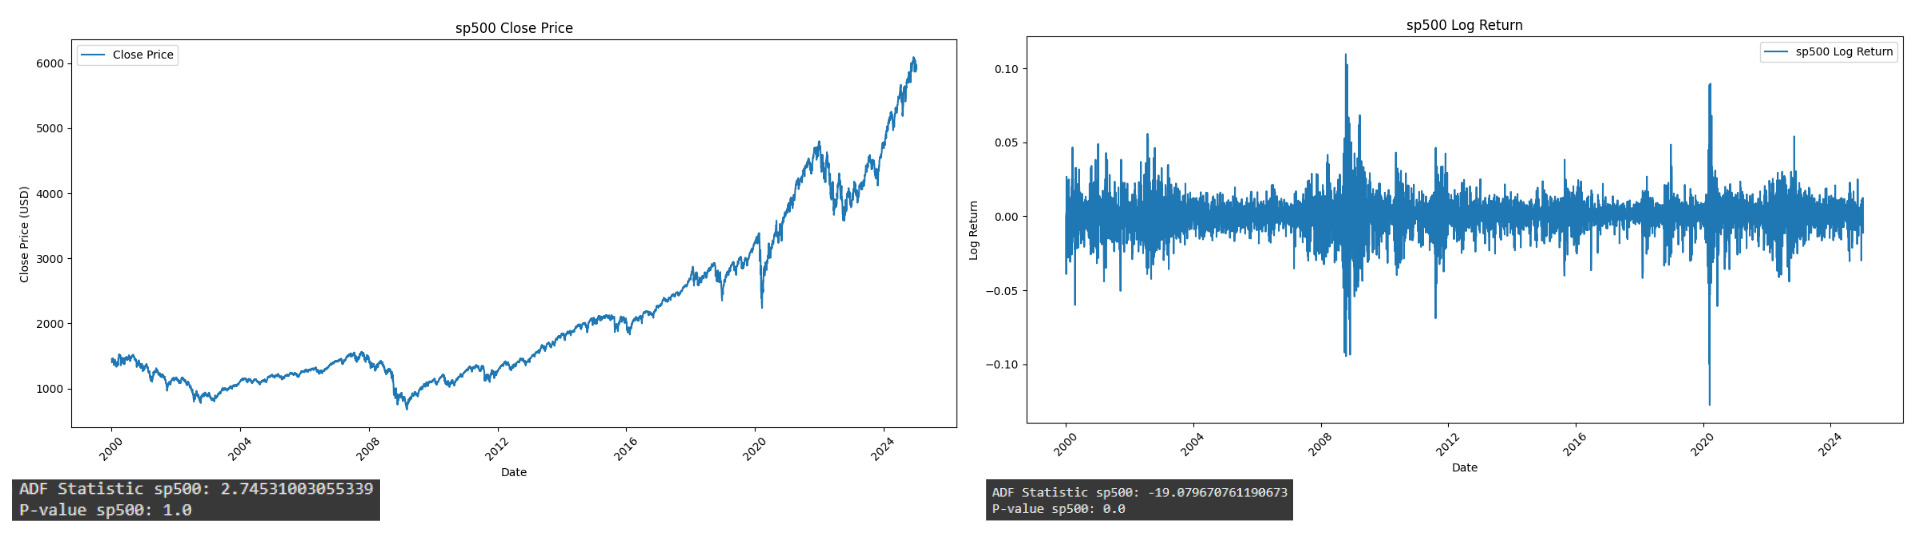
\includegraphics[width=1\textwidth]{Machine_learning_thesis/Images/Log returns.png}
    \caption{Log returns of the S\&P 500.} 
    \label{fig:Log returns}
\end{figure}
Log returns are then further differentiated in the seasonal order to eliminate any remaining seasonality, by applying the following transformation: 
\[
\nabla_s r_t = r_t - r_{t-s}
\]

\subsubsection{ML preprocessing}

After exctracting the residuals $\epsilon_t$ from the SARIMA model the series is preprocessed to generate pairs of input-output, which are appropriate for machine learning techniques. This involves using a sliding window technique to structure the residuals into a supervised learning problem. With this approach a window of k time-steps is defined, where each input sequence consists of k consecutive residuals:
\[
X_t = [\epsilon_{t-k}, \epsilon_{t-k+1}, \dots, \epsilon_{t-1}]
\]
and the corresponding target is defined as the residual at the next time-step:
\[
y_t = \epsilon_t
\]
For this study a window size of 10 was chosen, capturing around 2 weeks of trading days. The sliding windows transformation is applied sequentially across the residual series, generating a dataset of input-output pairs $(X_t, y_t)$. 

\subsubsection{Train, Test, Val split}

The 2 dataset are splitted into training, validation, and test to prevent data leakage when fine tuning the models and evaluating the performance on out-of-sample data.
The split are defined like this: 

For the S\&P500 dataset: 
\begin{itemize}
    \item \textbf{Training set}: January 2000 – December 2018
    \item \textbf{Validation set}: January 2019 - December 2021
    \item \textbf{Test set}: January 2022 - December 2025
\end{itemize}
For the EUR/USD dataset: 
\begin{itemize}
    \item \textbf{Training set}: January 2003 – December 2018
    \item \textbf{Validation set}: January 2019 - December 2021
    \item \textbf{Test set}: January 2022 - December 2025
\end{itemize}
The 3 split are done in such a way to preserve the chronological order of financial time series, ensuring that the model is trained on historical data, validated on intermediate periods, and tested on the most recent observations

\subsubsection{Data scaling}

To ensure that the ML models perform optimally and do not become biased toward any particular feature due to differences in scale between the training and testing set, both datasets are scaled using the Min-Max Scaler, which converts the data into a range between 0 and 1, helping the models to converge and be more stable, by applying the transformation:
\[
X_{\text{scaled}} = \frac{X - X_{\text{min}}}{X_{\text{max}} - X_{\text{min}}}
\]
where: 
\begin{itemize}
    \item \( X \) are the original feature values
    \item \( X_{\text{min}} \)is the minimum value of the feature in the dataset
    \item \( X_{\text{max}} \)is the maximum value of the feature in the dataset
    \item \( X_{\text{scaled}} \) are the scaled feature values, now in the range [0, 1].
\end{itemize}
To avoid data leakage the scaler is fitted exclusively on the training set to compute the parameters $X_{min}$ and $X_{max}$, which are then reused to transform both the validation and the testing sets.


\section{Capturing Linear Dependencies with SARIMA}
\subsection{SARIMA Model Selection}
The parameters that define the Seasonal AutoRegressive Integrated Moving Average (SARIMA) model are $(p,d,q) (P,D,Q)_S$, where:
\begin{itemize}
    \item \( p, d, q \) are the non-seasonal AR, differencing, and MA orders.
    \item \( P, D, Q \)are the seasonal AR, differencing, and MA orders.
    \item \( S \)is the seasonal period 
\end{itemize}
Tuning the parameters of the model requires an iterative procedure, which will be detailed below:

\textbf{Step I: Stationarity Assessment}

The first step in fine-tuning the model is to make sure the time series is stationary, which i checked by using the Augmented Dickey-Fuller (ADF) test on the log returns of the original time series.  Because the p-value is below the significance level of 0.01 (Figure \ref{fig:Log returns}), the ADF test revealed that the series was already stationary in its non-seasonal component (thus, no additional differencing was required, i.e., $d=0$). By looking at the sesonal components of the dataset with different time period (Figure \ref{fig:Seasonal components}) generated by decomposing the into trend, seasonal, and residual components, we can observe notable seasonal patterns across various cyclic intervals. 
\begin{figure}[H]
    \centering
    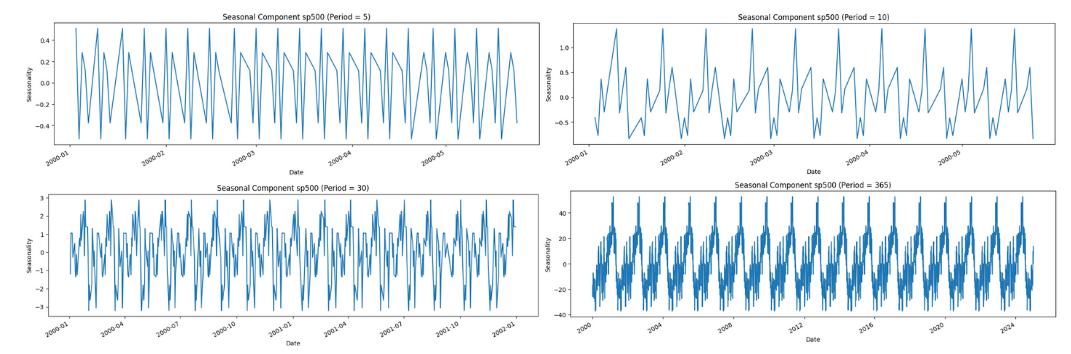
\includegraphics[width=0.9\textwidth]{Machine_learning_thesis/Images/seasonal components.png}
    \caption{Seasonal components of the S\&P 500 for different time periods.} 
    \label{fig:Seasonal components}
\end{figure}
I ultimately selected a seasonal period of $S=5$  to align with the 5-day trading week structure of financial markets.  While alternative seasonal interval were tested, $S=5$ was chosen, since it yielded a superior performance both on the test set and on the training set.  This choice is further supported by the literature: Hyndman \& Athanasopoulos \cite{Hyndman2018} claim that overly complicated seasonal models rarely enhances forecasts for fnancial data, because short-term cyclicality influenced by investor activity is frequently more significant than rigid calendar-based seasonality.

\textbf{Step II: ACF and PACF Analysis}

To find possible values for the seasonal and non-seasonal parameters, I then examined the Autocorrelation Function (ACF) and Partial Autocorrelation Function (PACF) plots (Figure \ref{fig:ACF and PACF}).
\begin{figure}[H]
    \centering
    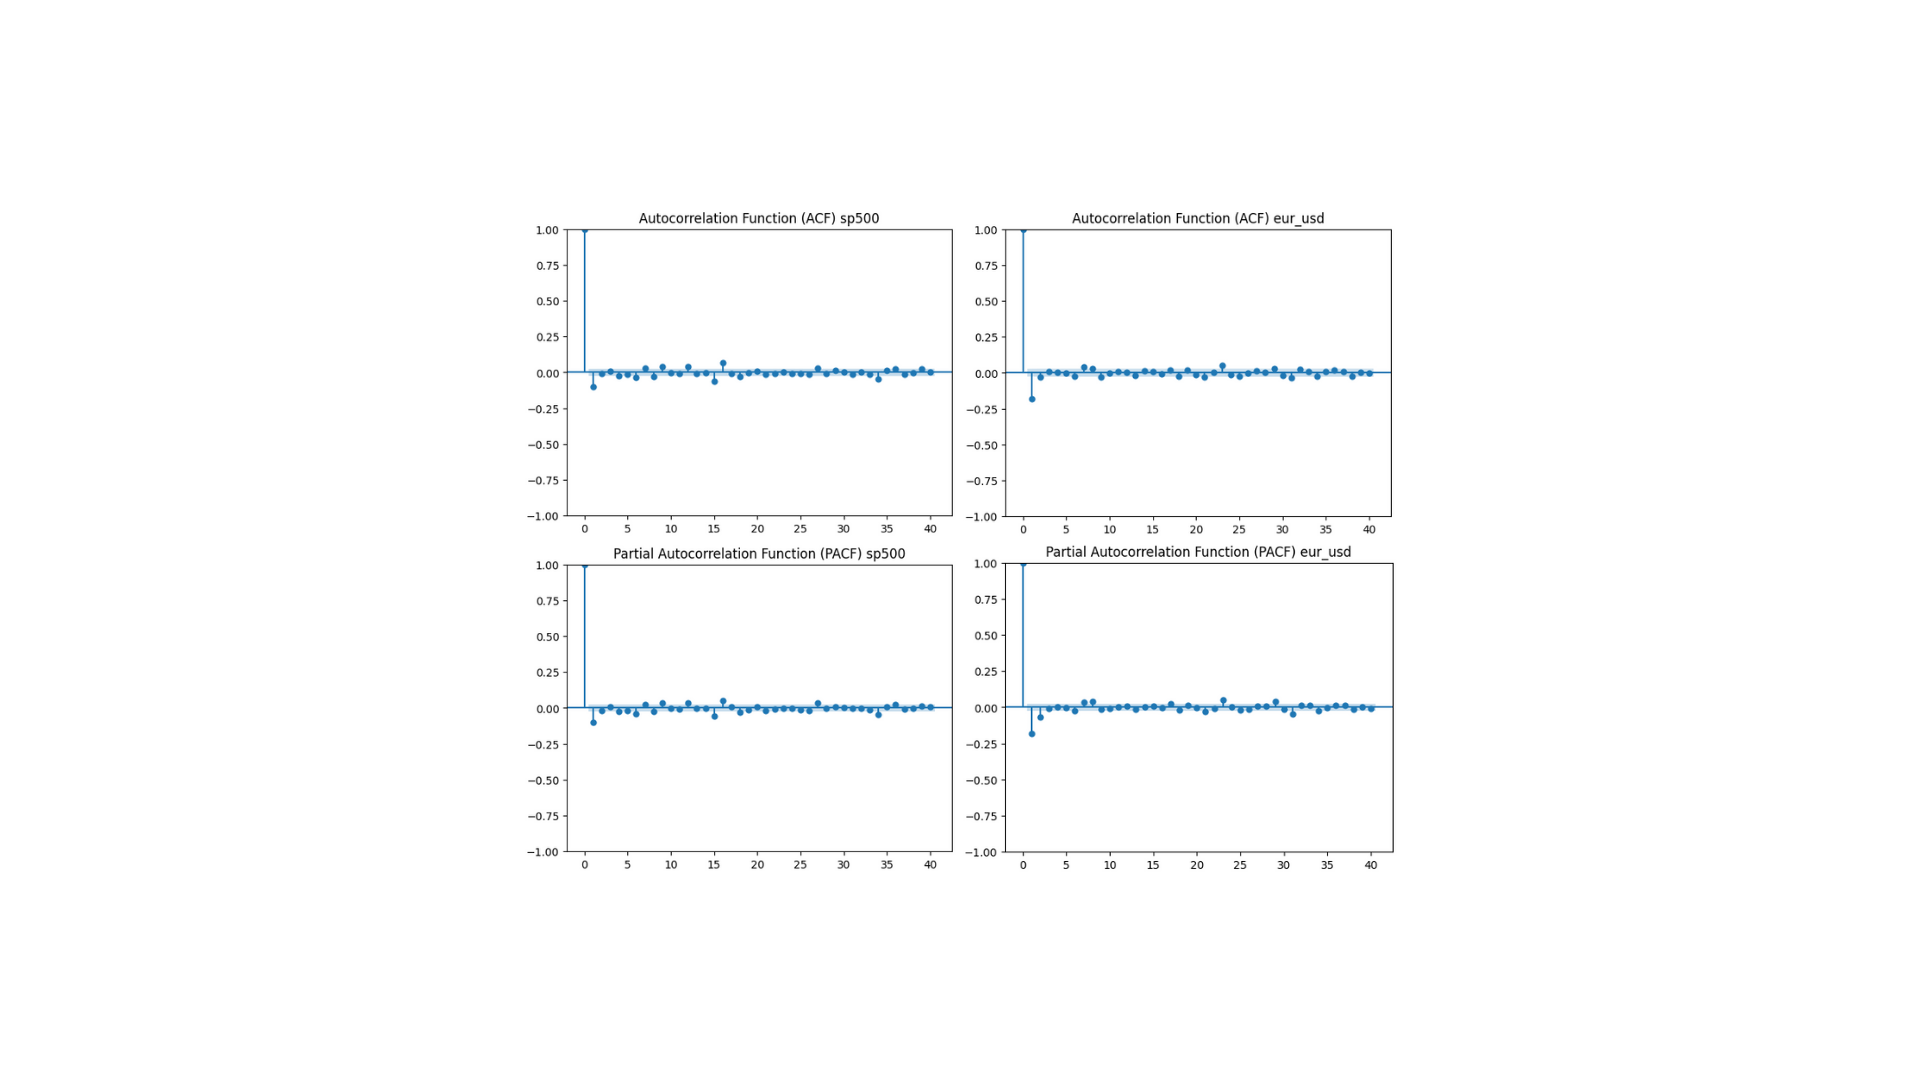
\includegraphics[width=0.9\textwidth]{Machine_learning_thesis/Images/ACF and PACF.png}
    \caption{Autocorrelation Function and Partial Autocorrelation Function.} 
    \label{fig:ACF and PACF}
\end{figure}
Although lag 1 is the dominant feature in both plots (for both datasets) including lag 2 improved the model's ability to capture additional temporal dependencies without overfitting. This decision was validated by testing every possible combination of parameters. The final model was configured with $p=2$, $q=2$, $P=0$, and $Q=0$, as these settings yielded the best performance.

\subsection{Model fitting and rolling forecasting} 
After identifying the optimal parameters, I fitted the SARIMA model using the following configuration for both datasets:
\begin{verbatim}
model = ARIMA(history, order=(2, 0, 2), trend='n', seasonal_order=(0, 1, 0, 5)).fit()
\end{verbatim}
To ensure accurate out-of-sample prediction and to simulate a real world scenario a \textbf{rolling forecasting} approach was implemented. This method iteratively trains the model using an expanding window of historical data, generate predictions on the next time step and updates the training set with the most recent observed value (Figure \ref{fig:Rolling forecas}).
 \begin{figure}[H]
    \centering
    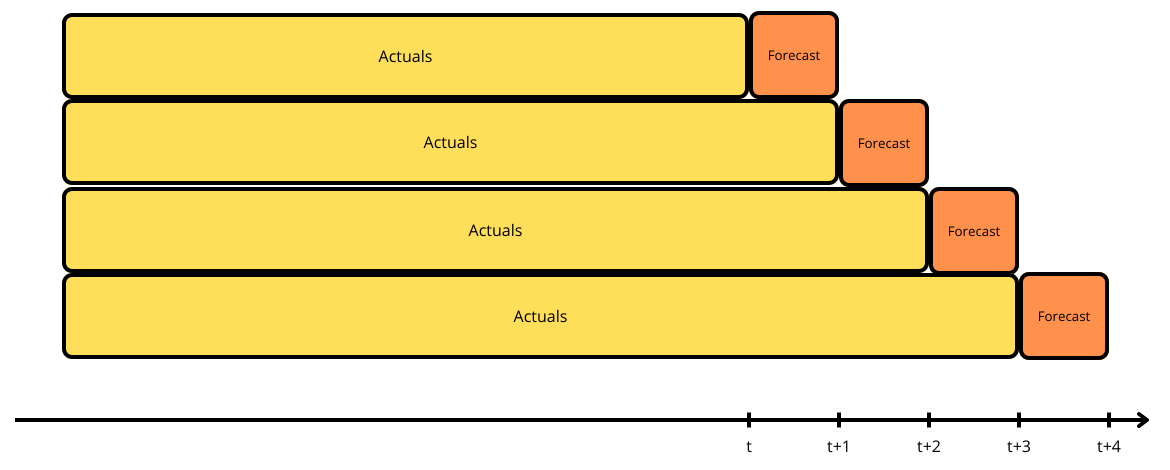
\includegraphics[width=0.8\textwidth]{Machine_learning_thesis/Images/Rolling forecast.png}
    \caption{Rolling forecast.} 
    \label{fig:Rolling forecas}
\end{figure}
Predictions were generated for both the training and validation sets. The validation set predictions are particularly critical, bacause they reflect the model's ability to capture temporal dependencies in unseen data, therefore, the residuals computed from the validation set will contain any non linear patters that the SARIMA model was not able to explain. This residuals will later be used to train an ensemble of ML models, that will capture the nonlinear dynamics in the residuals, in order to predict the residuals on the test set.
 \begin{figure}[H]
    \centering
    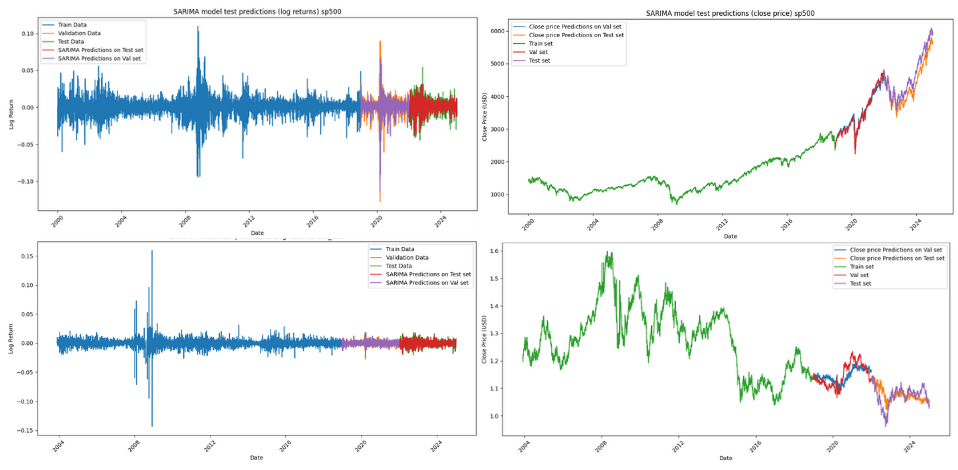
\includegraphics[width=0.8\textwidth]{Machine_learning_thesis/Images/SARIMA predictions.png}
    \caption{SARIMA predictions on the Validation and Test set.} 
    \label{fig:SARIMA predictions}
\end{figure}

\subsection{Residual Extraction}
Residuals were computed as the difference between the observed closing prices and the SARIMA model’s predicted values, transformed back to the original price scale. This choice was motivated by the need to improve interpretability, as residuals in the original price domain directly quantify deviations from actual market prices, making them more relevant for the analysis, as the objective is to predict prices rather than returns. Furthermore, non-linear relationships that would be smoothed out in log returns are preserved while working in the price domain, which enables later machine learning models to better identify patterns that SARIMA is unable to explain. This method of estimating residuals guarantees that the mistakes represent actual market discrepancies, allowing for more precise forecasts and adjustments in the following modeling stages. Since the SARIMA model was trained on log returns (to stabilize variance and achieve stationarity), the predictions were first converted from log returns to closing prices, by applying the inverse transformation:
\[
\hat{P}_t = P_{t-1} \cdot \exp(\hat{r}_t)
\]
where: 
\begin{itemize}
    \item \( P_{t-1} \) is the observed closing price at $t-1$
    \item \( \hat{P_t} \) is the predicted closing price at time $t$.
\end{itemize}
then the residuals are computed using the formula: 
\[
\epsilon_t = P_t - \hat{P}_t
\]
 \begin{figure}[H]
    \centering
    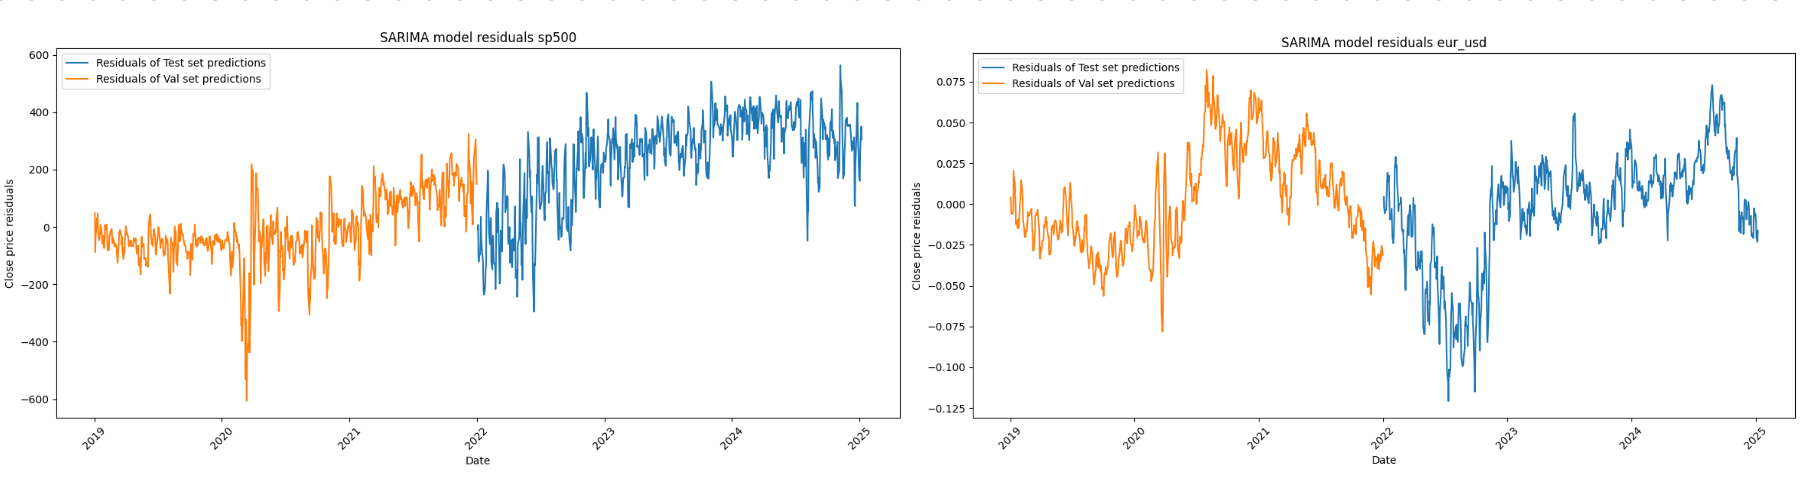
\includegraphics[width=0.8\textwidth]{Machine_learning_thesis/Images/SARIMA residuals.png}
    \caption{SARIMA residuals on the Validation and Test set.} 
    \label{fig:SARIMA residuals}
\end{figure}

\section{Residual Learning for Non-Linear Dependencies}

\subsection{Model Selection}
An ensemble of machine learning (ML) and deep learning (DL) models was used to capture the non-linear dependencies in the residuals of the SARIMA model. The ensemble includes a linear booster model, a Convolutional Neural Network (CNN), a Long Short-Term Memory (LSTM) network, and two hybrid CNN-LSTM architecture. 

\subsubsection{Linear Booster model}

A linear tree, implemented in the \texttt{linear-tree} library (available on GitHub: \url{https://github.com/cerlymarco/linear-tree}) is a machine learning technique that combine the learning ability of Decision Tree with the predictive and explicative power of Linear Models. Unlike traditional tree-based methods, which recursively split the feature space into disjoint regions (leaves) and assign a constant predictions (e.g., the average target value) within each region, a linear booster instead fits a linear model within each leaf of the tree. This approach allows the model to capture linear relationships within subsets of the data, making it particularly useful for scenarios where the relationship between features and the target variable is not purely nonlinear. The primary reason I've chosen this implementation of the Tree Boosting model, instead of a more popular option such as XGBoost, is for its ability to to extrapolate predictions outside the range of the training data. Traditional tree-based models instead are intrinsically constrained in their capacity to extrapolate since they rely on region-specific constant predictions, meaning that predictions are constrained to the range of target values observed during training, making them unsuitable for tasks requiring predictions beyond this range.
 \begin{figure}[H]
    \centering
    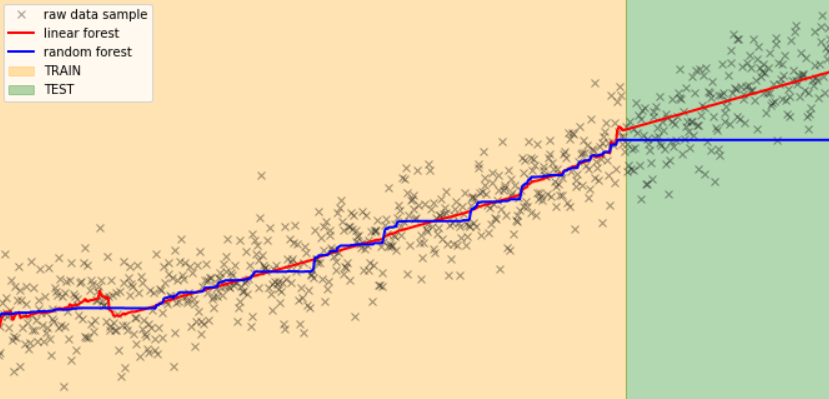
\includegraphics[width=0.8\textwidth]{Machine_learning_thesis/Images/Linear forest.png}
    \caption{Comparison of performance on unseen data between Linear Forest and Random Forest.} 
    \label{fig:Linear Forest}
\end{figure}

\subsubsection{LSTM model}

A Long Short Term model was chosen to capture the nonlinear dependencies of residuals due to their ability to identify long-term patterns and non-linear connections in sequential data. The gating mechanisms: the forget gate, input gate, and output gate enable the model to selectively retain and update information over long time horizons. Many architecture have been tested, but the one that achieved the best results is the one presented below.
 \begin{figure}[H]
    \centering
    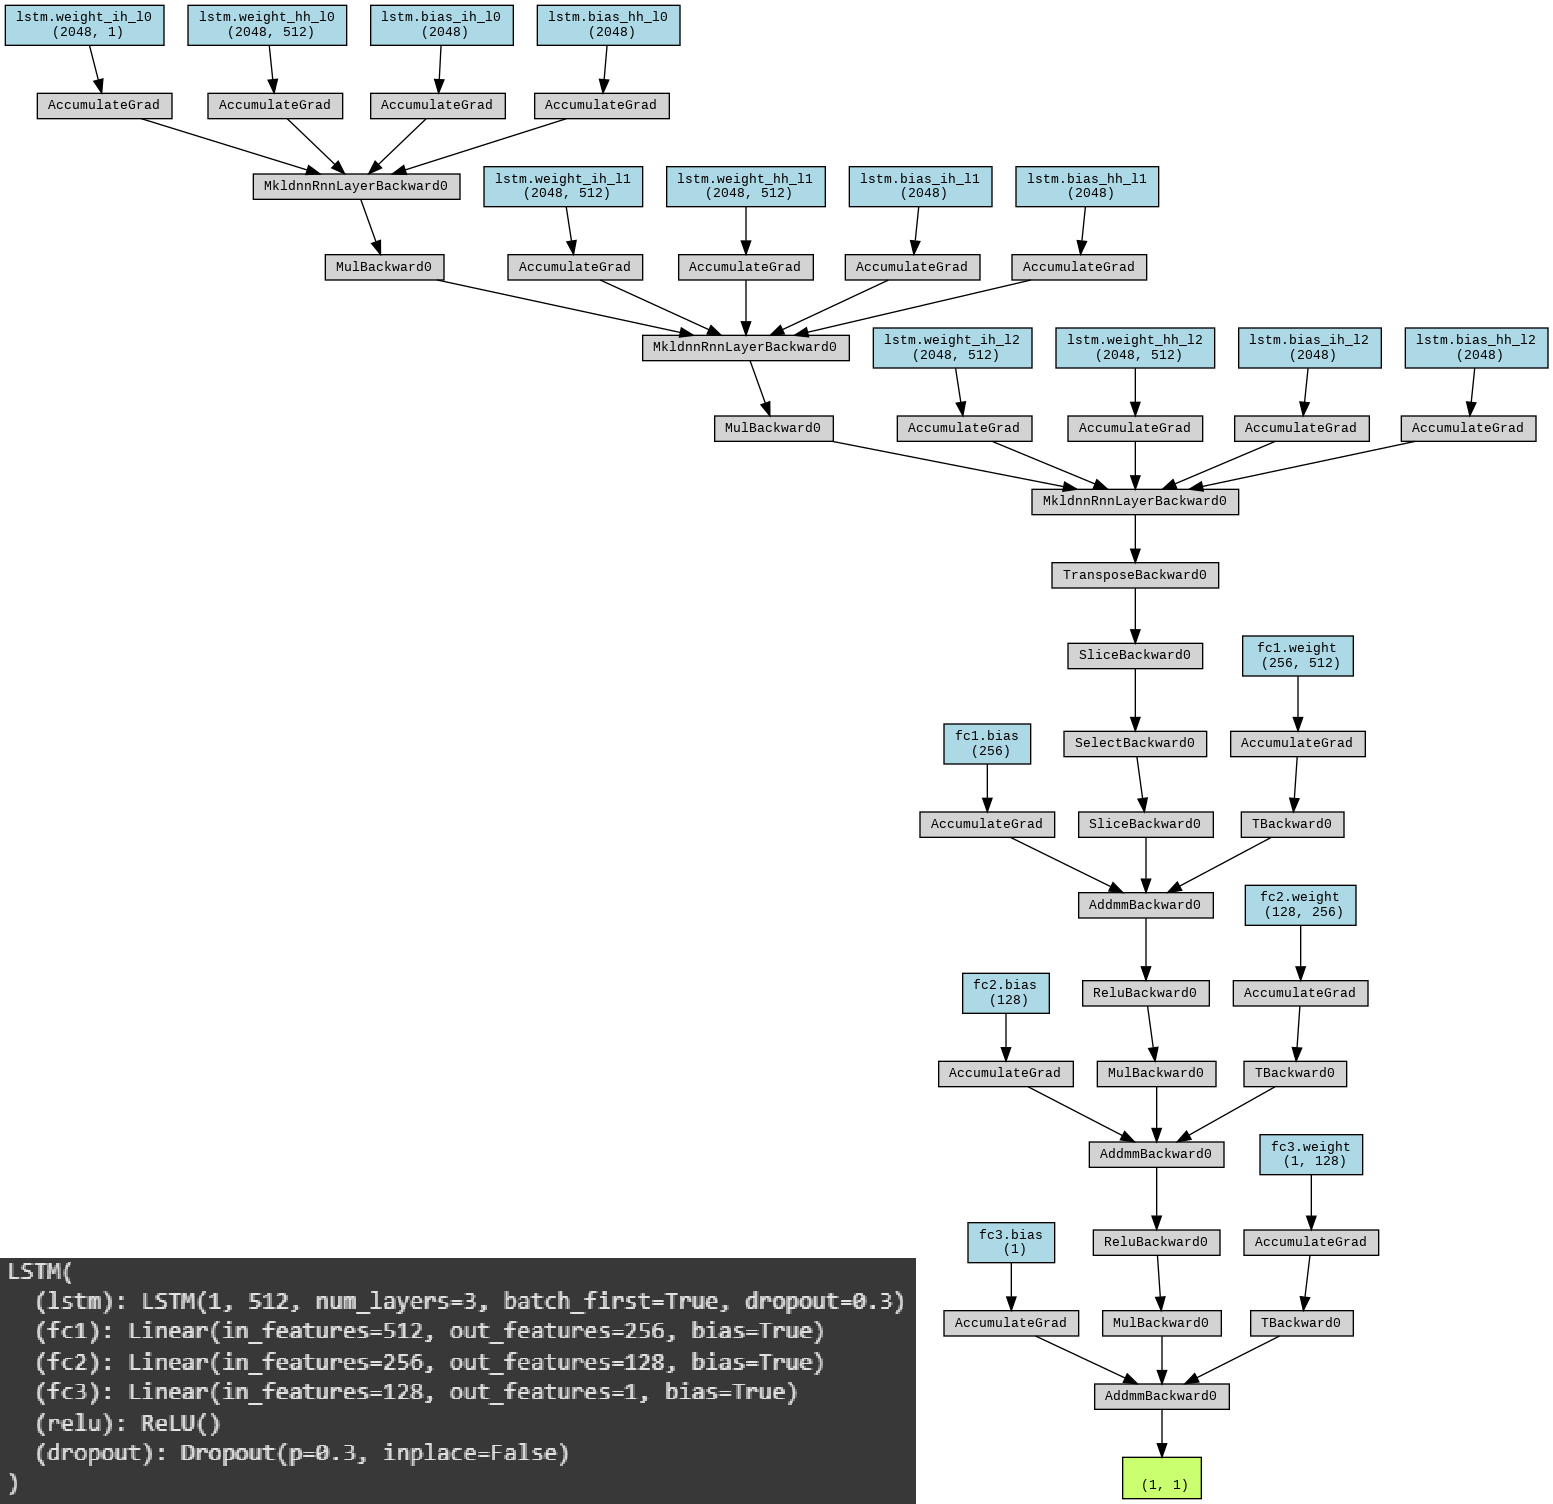
\includegraphics[width=0.8\textwidth]{Machine_learning_thesis/Images/LSTM architecture.png}
    \caption{LSTM architecture.} 
    \label{fig:LSTM architecture}
\end{figure}
The Neural Network is composed of three stacked LSTM layer stacked, where each one has 512 hidden units. This stacked configuration allows the model to capture hierarchical temporal patterns, With upper layers modeling long-term trends and lower layers learning short-term dependencies. A dropout rate of 0.3 is being used between each LSTM layers to prevent overfitting and guarantee strong generalization to residual data that are noisy. The LSTM output is then passed through a series of fully connected (FC) layers that gradually lower dimensionality, with the third and final layer that maps 128-dimensional representation into a sigle output, producing the residual prediction. A ReLU activation is used in the first two FC layers to add non-linearity, which helps the model identify intricate correlations in the residuals. Other dropout layers, with a probability of 0.3, are applied after each FC layer to further regularize the network. 

\subsubsection{CNN model}

CNNs use convolutional kernels over temporal segments to identify significant features such as local trends, seasonal effects, or abrupt shifts within the residuals. Convolutional layers are often stacked together enabling the model to learn hierarchical representations, where simple patterns are progressively combined into more abstract features capturing complex, nonlinear interactions. Below is presented the architecture of the model.
 \begin{figure}[H]
    \centering
    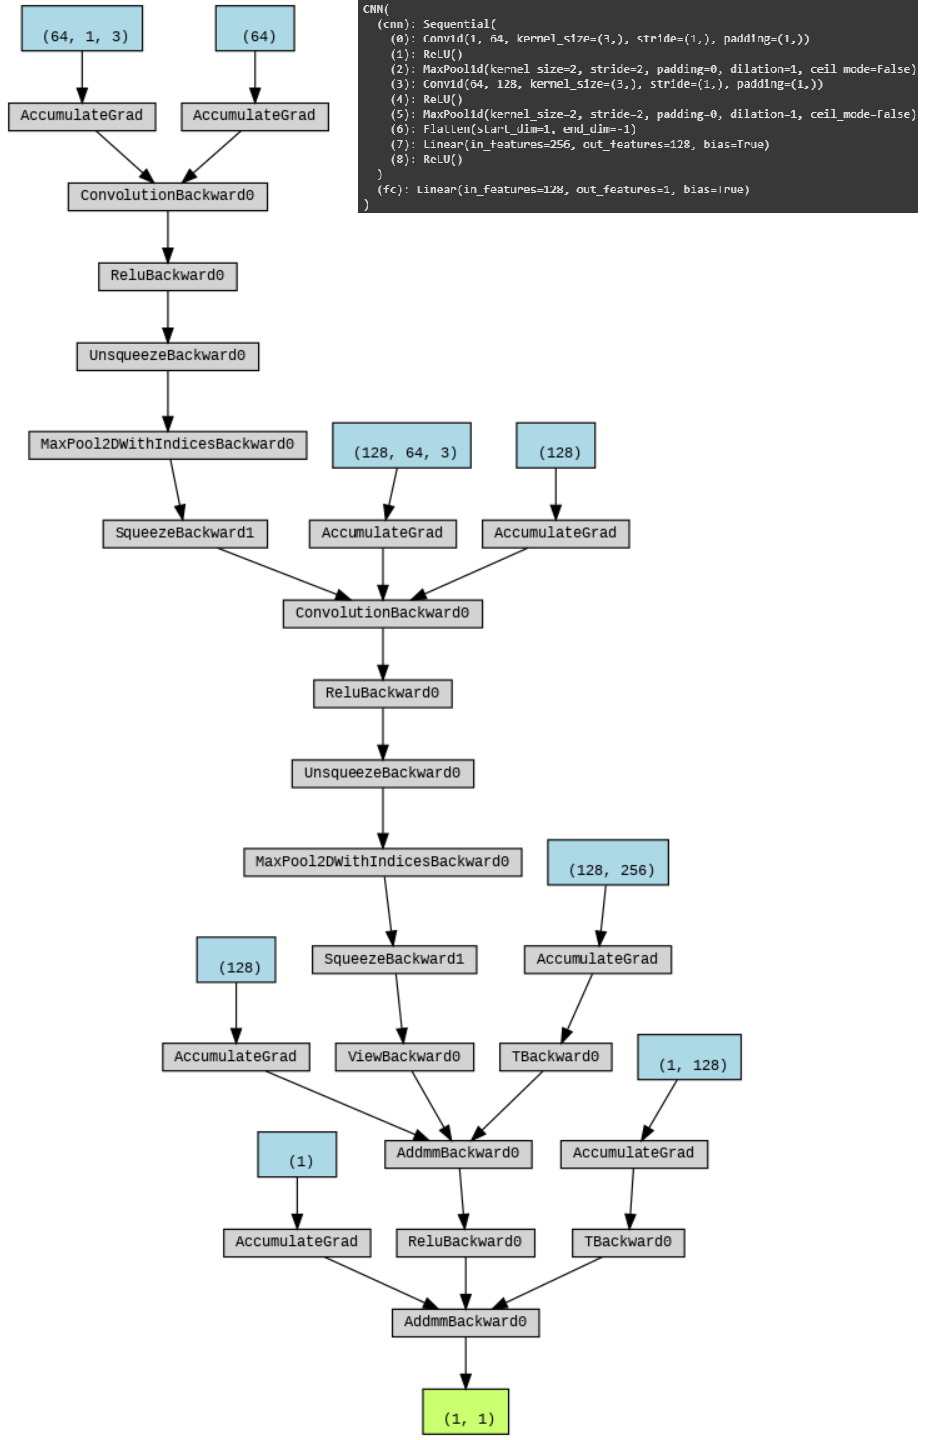
\includegraphics[width=0.8\textwidth]{Machine_learning_thesis/Images/CNN architecture.png}
    \caption{CNN architecture.} 
    \label{fig:CNN architecture}
\end{figure}
The architecture consist of two layers of 1D convolutions, which progressively expand the feature map using a kernel of size 3, stride 1, and padding of 1 to preserve the temporal dimensions. Each conavolutional layers is followed by a ReLu activation function, which introduces non linearity into the model, followed by a max pooling layer that downsamples the output by a factor of 2, reducing the sequence length while retaining key features. After reaching a feature map of 128, it gets flattened into a one-dimensional vector. This vector is passed through a fully connected (FC) network, which incudes two linear layers and a ReLu activation function in between, that progressively reduce the dimensionality of the flattened vector into a single output value, generating the final prediction. 

\subsubsection{CNN LSTM hybrid architecture}


CNNs are good at capturing local patterns and spatial correlations extracting high-level feature representations sliding convolutional filters to sequential data. However, long-term dependencies are not explicitly modeled by CNNs alone. By using gating mechanisms (forget, input, and output gates) to selectively store or discard information, LSTMs, on the other hand, are specifically made to handle long-term dependencies in sequential data. For this reasons several studies suggest that combining the two previously described models into a single architecture can improve forecasting performance by efficiently capturing both spatial and temporal patterns in time series data \cite{zhao2017}. In this study two hybrid architecture have been proposed: a Parallel CNN-LSTM Architecture and a Sequential CNN-LSTM Architecture, which will be presented below.
 \begin{figure}[H]
    \centering
    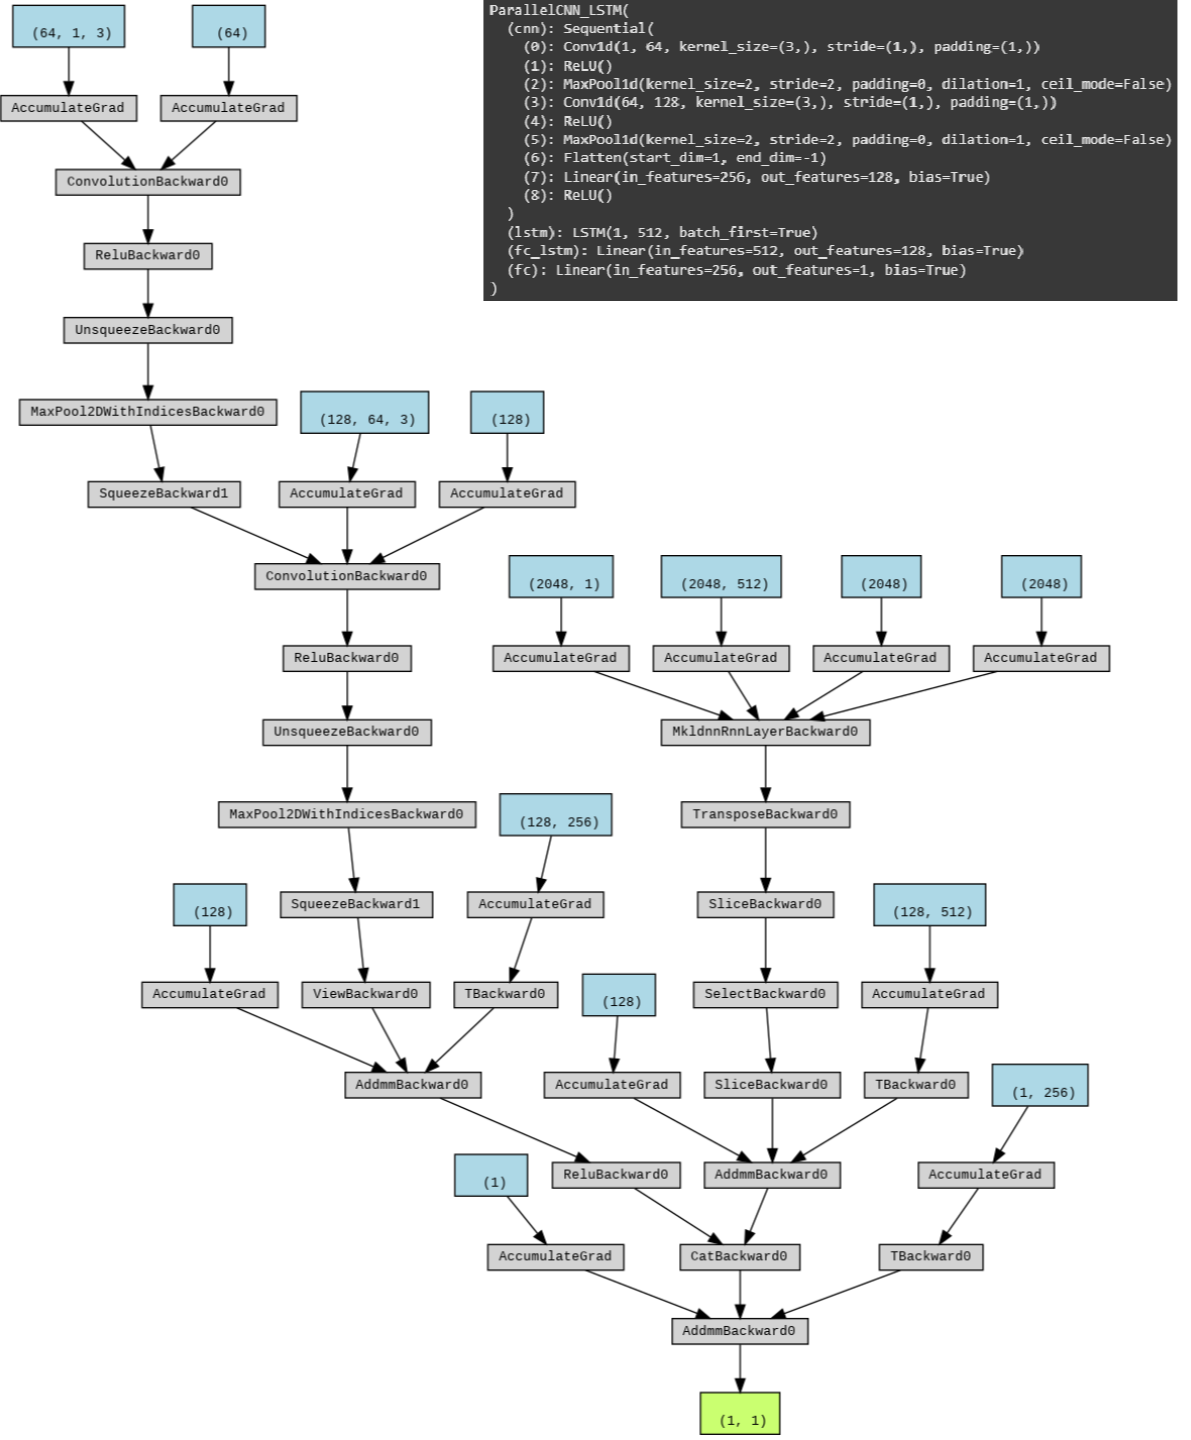
\includegraphics[width=0.8\textwidth]{Machine_learning_thesis/Images/ParallelCNN_LSTM architecture.png}
    \caption{Parallel CNN LSTM architecture.} 
    \label{fig:Parallel CNN LSTM architecture}
\end{figure}
The model architecture has two branches: a CNN branch and a LSTM branch, Both branches process the same input independently and later merge their outputs. The architecture of the two branches is identical of the two previous model, the output of each branch is then concatenated into a single tensor along the feature dimension, and it is fed into a Final Fully Connected Layer, which maps the features into a single output value.
 \begin{figure}[H]
    \centering
    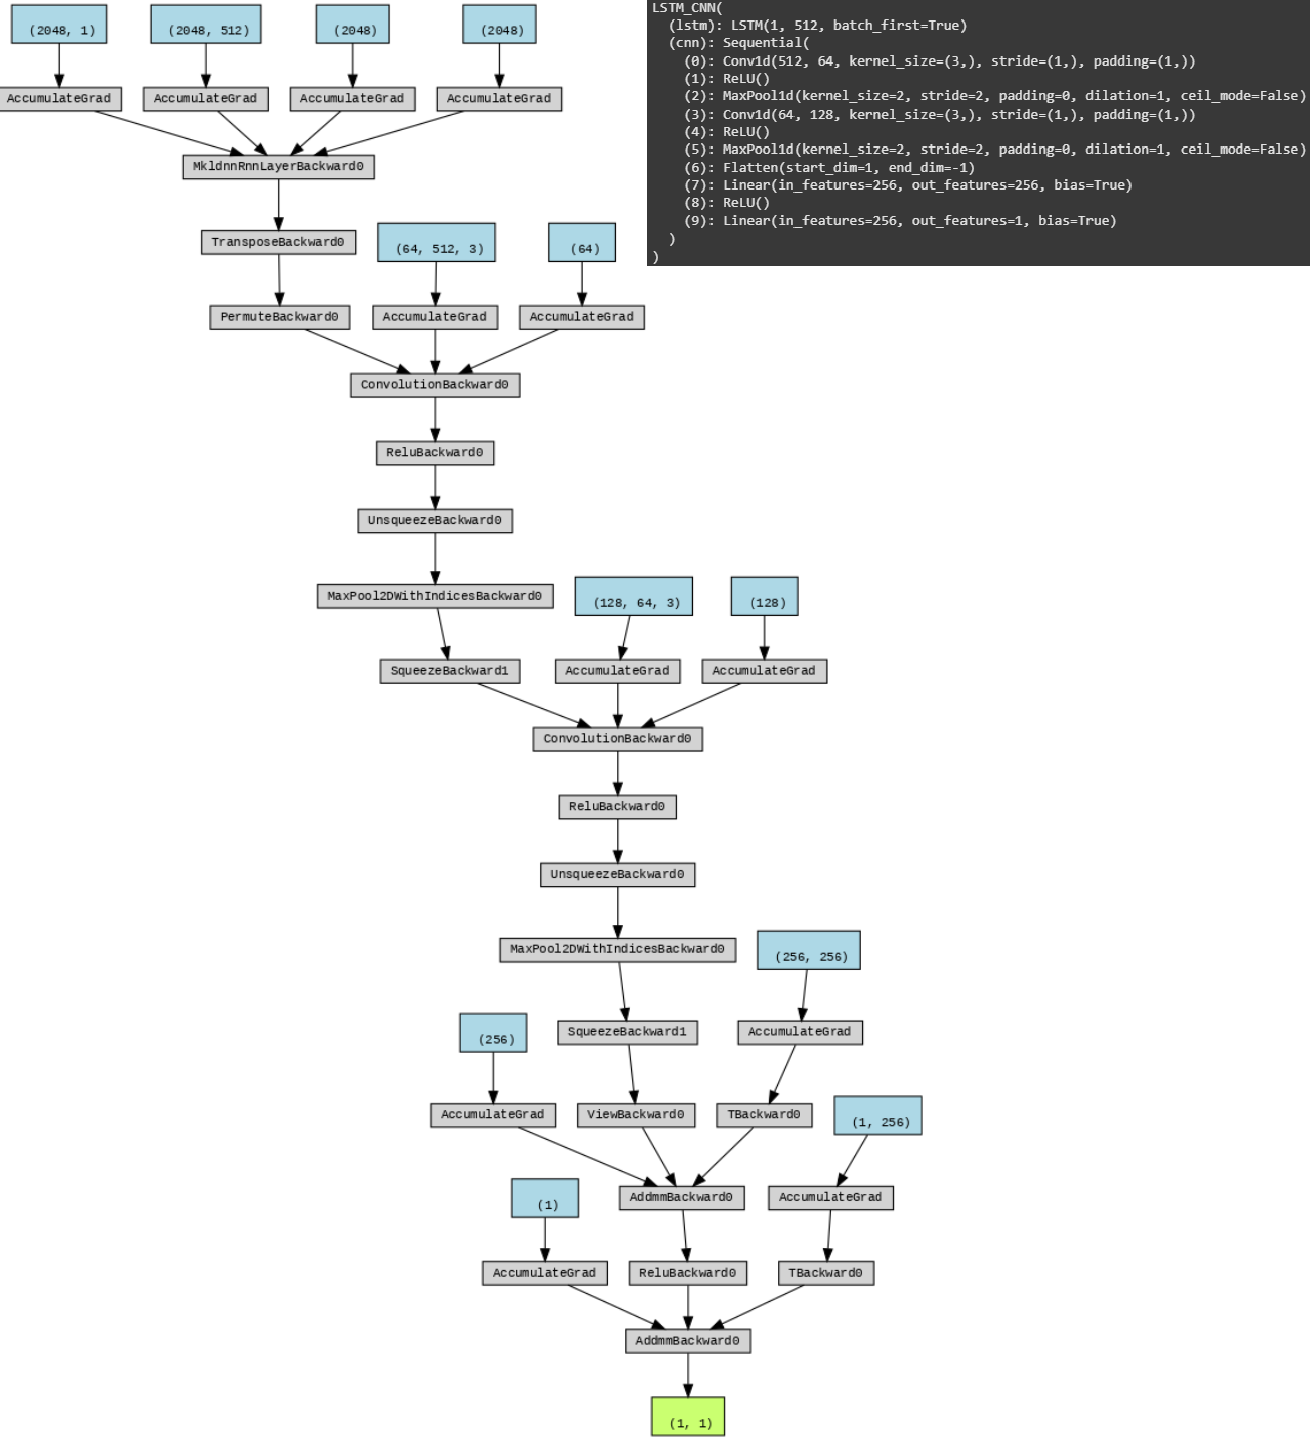
\includegraphics[width=0.8\textwidth]{Machine_learning_thesis/Images/SequentialLSTM_CNN architecture.png}
    \caption{Sequential LSTM CNN architecture.} 
    \label{fig:Sequential LSTM CNN architecture}
\end{figure}
This model architecture combines an LSTM with a CNN in a sequential manner by first processing the input through an LSTM to capture long-term temporal dependencies, and then feeding the LSTM’s output into a CNN to extract local, high-level features, the final layers are two stacked Fully Connected Layers which maps the flattened features extracted by the Convolutional layers (see architecture \ref{fig:CNN architecture}) into a single prediction. 

\subsection{Training and Validation process}
The training and validation process consisted of two distinct strategies tailored to the different components of the ensemble.

\subsubsection{Linear Booster:}
The linear booster was tuned using \texttt{arm mango}, a Bayesian optimization library to automatically tune the model hyper-parameters evaluating the accuracy on the Validation set. Bayesian Optimization is a powerful approach for solving black-box optimization problems efficiently, rather than trying every possible input. The way this optimization technique works can be summarized by the following steps: 
\begin{itemize}
    \item \textbf{Initialization}: a few hyper-parameter configurations are randomly selected,  and the model is assessed with these configurations and the corresponding validation accuracy is recorded, which will serve as the foundation for building the surrogate model.
    \item \textbf{Surrogate Model Construction}: With the initial observations a  a probabilistic surrogate model (a Gaussian Process in this case) is constructed, the model approximates the relationship between the hyper-parameters and the model's performance on the Validation set
    \item \textbf{Acquisition Function Application}: An acquisition function is then employed to determine the next set of hyper-parameters to evaluate, balancing exploration , which are the regions where the surrogate model is uncertain and exploitation, targeting regions where the model predicts high accuracy
    \item \textbf{Candidate Selection}: the next hyper-parameters configuration to be selected is the one that maximizes the acquisition function
    \item \textbf{Evaluation and Update}: the selected hyper-parameter configuration is then used to train the model and its performance is evaluated on the validation set
    \item \textbf{Iteration}: repeat step 3 to 5 for the predefined number of iteration. 
\end{itemize}
After the tuning process, the best hyper-parameters found were as follows:

\textbf{For the S\&P500 dataset:}\begin{verbatim}
{
  "n_estimators": 180,  
  "max_depth": 10,  
  "min_samples_split": 10,  
  "min_samples_leaf": 0.01
}
\end{verbatim}
\textbf{For the EUR/USD dataset:}\begin{verbatim}
{
"n_estimators": 5,  
"max_depth": 11,  
"min_samples_split" : 5, 
"min_samples_leaf" : 0.01
}
\end{verbatim}
Both configurations employ a Ridge regressor with an \texttt{alpha} value of 2 as the base estimator for the linear booster. The Ridge regressor was chosen since it incorporates L2 regularization, which helps to control the magnitude of the regression coefficients stabilizing the estimates, making the model less sensitive to noise. An \texttt{alpha} of 2 provided a good balance between bias and variance.
Below we can see the prediction on the Test residuals.
 \begin{figure}[H]
    \centering
    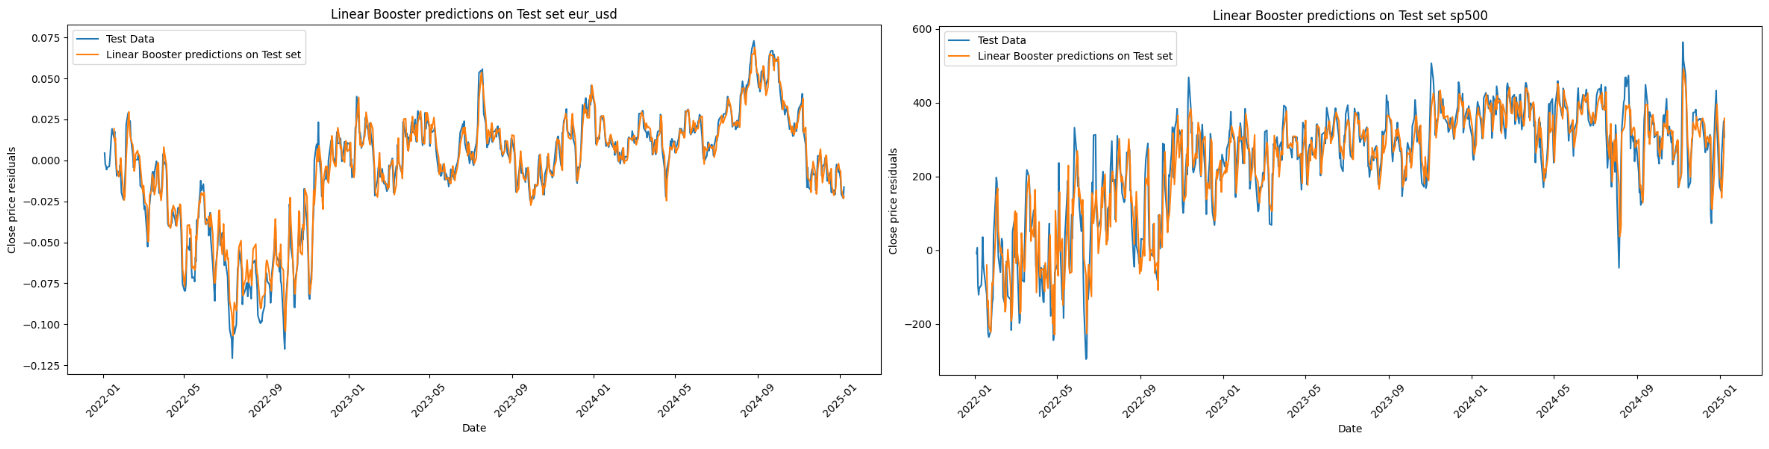
\includegraphics[width=1\textwidth]{Machine_learning_thesis/Images/Linear Boost predictions.png}
    \caption{Linear Boost predictions.} 
    \label{fig:Linear Boost predictions}
\end{figure}

\subsubsection{Neural Networks}
The neural networks were trained using a structured pipeline designed to optimize convergence and generalization. The training process was conducted on a T4 GPU, leveraging its parallel processing capabilities and CUDA-accelerated tensor operations to enhance computational efficiency and reduce training time. The model were trained in batches using PyTorch's DataLoader utilities, which optimize memory management by loading sections of the dataset sequentially rather than the complete datasets at once. Training in batches is typical for neural network and in general deep learning models since it provides three main benefits: computational performance through parallelized matrix operations on GPU architectures, regularization by stochastic gradient noise, preventing over-fitting and memory feasibility by avoiding GPU VRAM limitations imposed by large datasets. The optimizer used was Adam, a  popular optimization algorithm,  which updates the model parameters using adaptive learning rates for each parameter, using the formula:
\[
\theta_t = \theta_{t-1} - \frac{\alpha\, \hat{m}_t}{\sqrt{\hat{v}_t} + \epsilon}
\]
where:
\begin{itemize}
    \item \(\theta_t\) is the model parameter at iteration \(t\).
    \item \(\alpha\) is the learning rate.
    \item \(\hat{m}_t\) is the bias-corrected first moment (mean of gradients), defined as $\hat{m}_t = \frac{m_t}{1 - \beta_1^t}$
    \item \(\hat{v}_t\) is the bias-corrected second moment (variance of gradients), defined as $m_t = \beta_1 \cdot m_{t-1} + (1 - \beta_1) \cdot g_t$
    \item \(\epsilon\) is a small constant for numerical stability, to prevent division by zero.
\end{itemize}
 A two-phase learning rate scheduler was integrated: an initial warm-up phase, during which the learning rate is linearly increased from zero to the target maximum value, to stabilize early gradient updates, which is followed by an adaptive annealing phase where the \texttt{ReduceLROnPlateau} scheduler monitored validation loss, if no progress was shown after 5 epochs the learning rate was decreased by a factor of 0.5, with a floor of $1 \times 10^{-7}$ for numerical stability. 
  \begin{figure}[H]
    \centering
    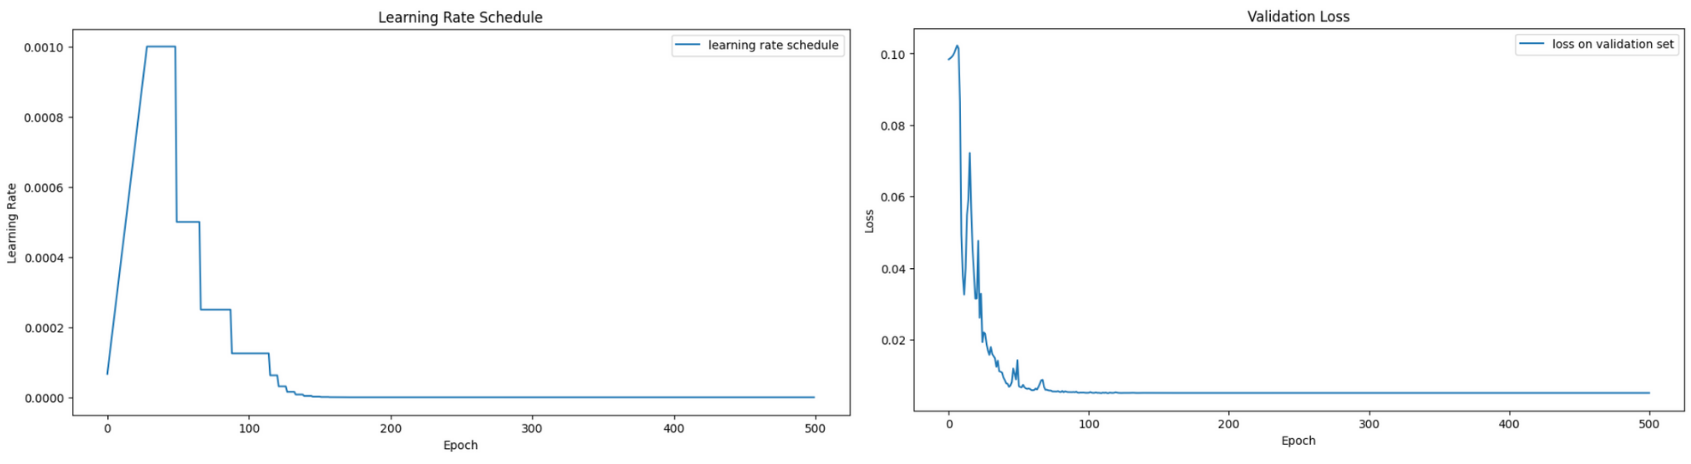
\includegraphics[width=1\textwidth]{Machine_learning_thesis/Images/NN training.png}
    \caption{Learning rate scheduling and Validation loss.} 
    \label{fig:NN training}
\end{figure}
Below we can see the prediction on the Test residuals.
  \begin{figure}[H]
    \centering
    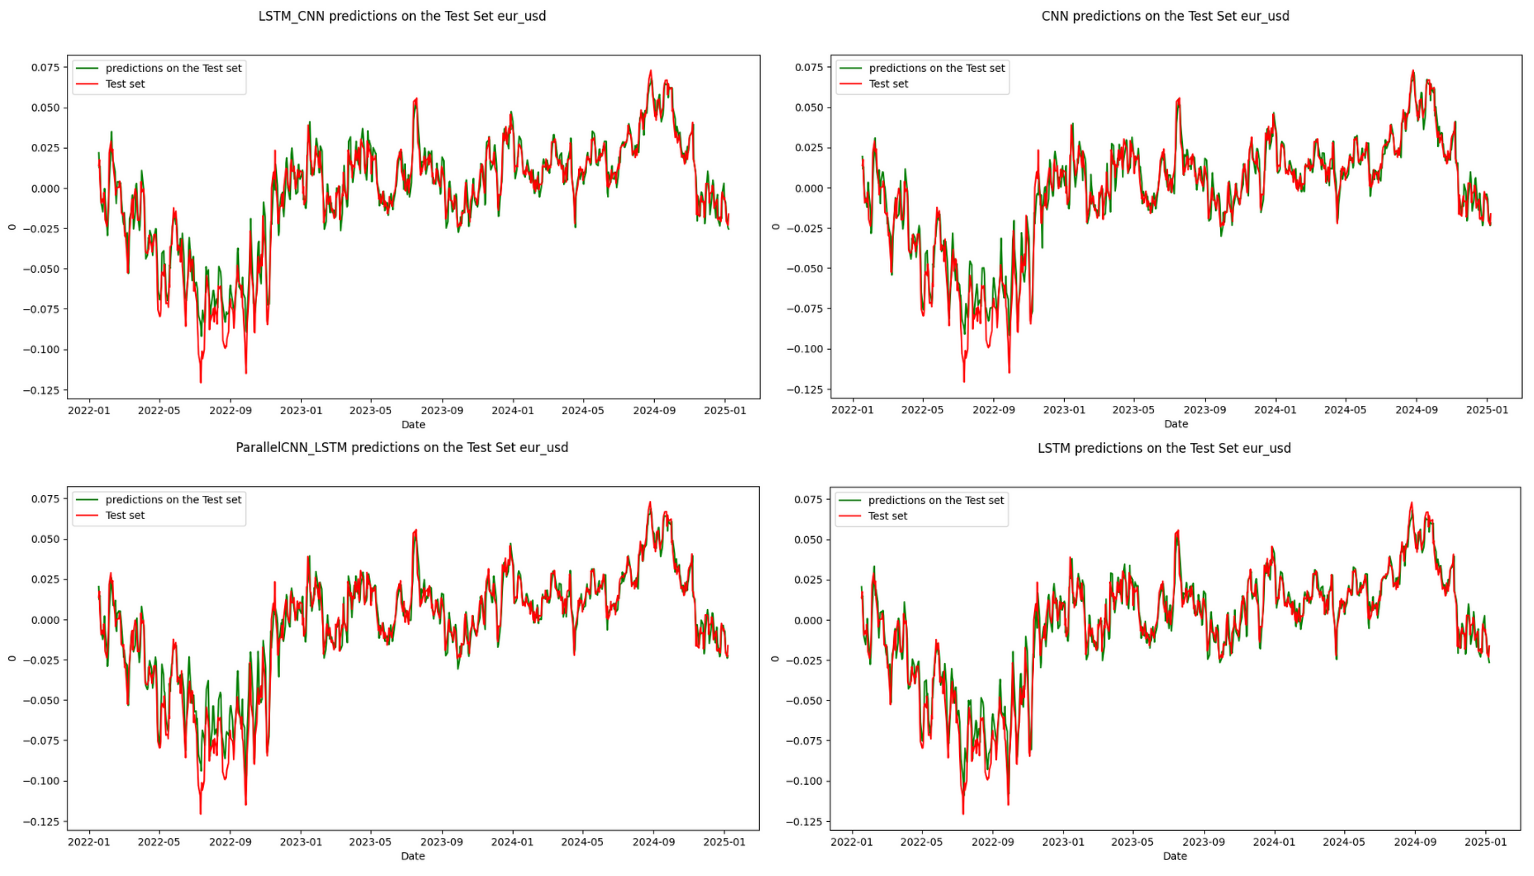
\includegraphics[width=1\textwidth]{Machine_learning_thesis/Images/NN predictions EURUSD.png}
    \caption{NN predictions on EUR/USD dataset.} 
    \label{fig:NN predictions EURUSD}
\end{figure}
  \begin{figure}[H]
    \centering
    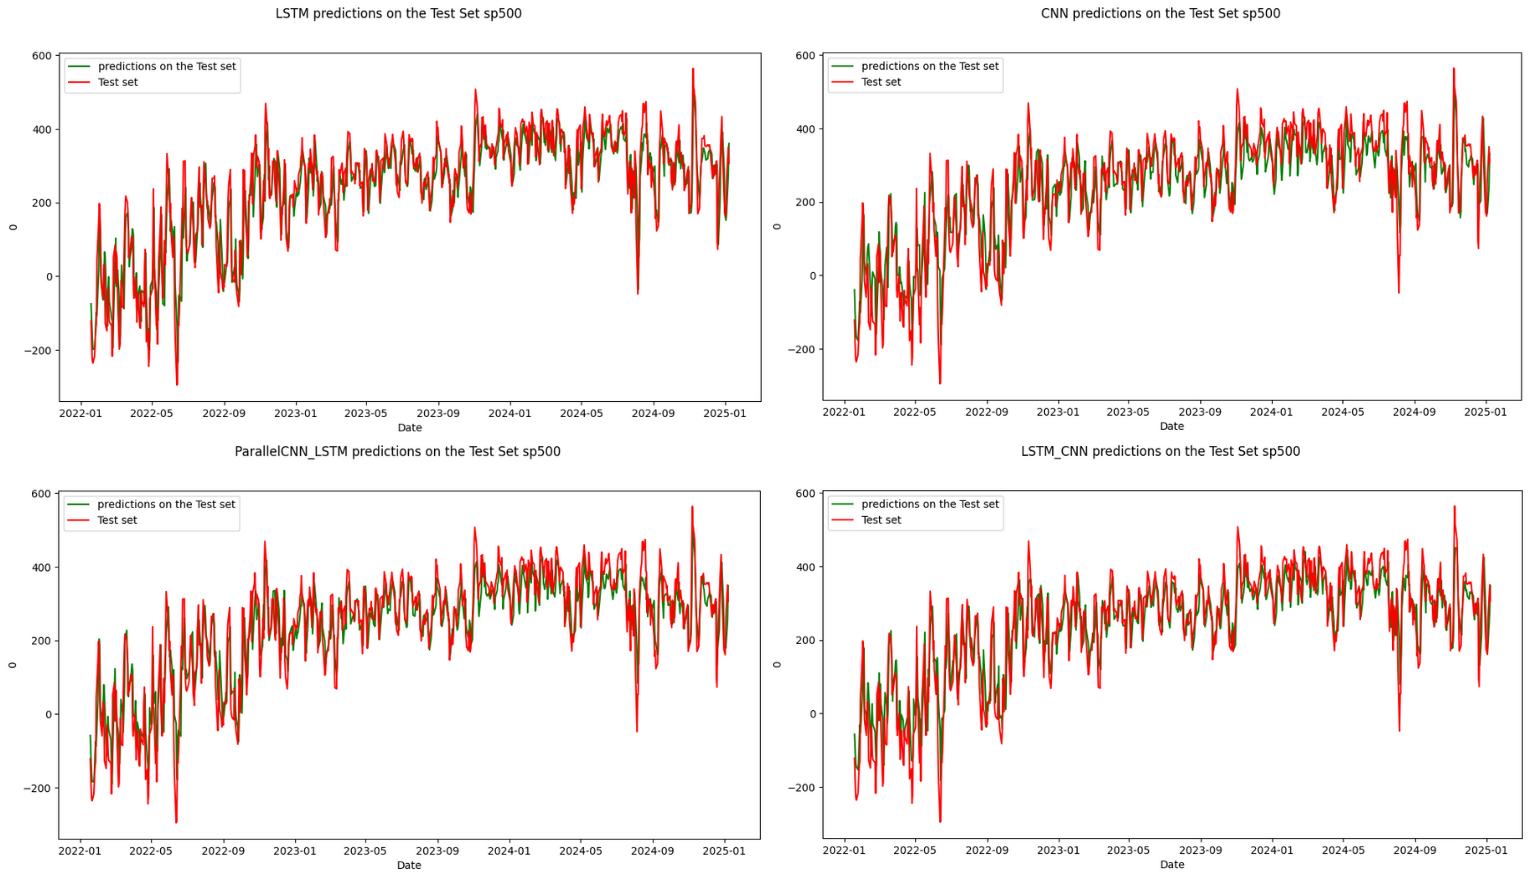
\includegraphics[width=1\textwidth]{Machine_learning_thesis/Images/NN predictions S&P500.png}
    \caption{NN predictions on S\&P500 dataset.} 
    \label{fig:NN predictions S&P500}
\end{figure}



\section{Arbitrated Dynamic Ensemble implementation}
The implementation of the ensemble technique (previously described in Section \ref{Arbitrated Dynamic Ensemble}) is available in the GitHub repository \url{https://github.com/andreadamiano/Machine_learning/tree/main/Project_code/ARIMA}. 

The ensemble technique operates in two distinct phases: an offline phase, in which the base models are used to generate the predictions and the corresponding errors are computed, and an online phase, in which the predictions are dynamically weighted employing a set of meta learner (Figure \ref{fig:ADE}).

\subsubsection{Offline phase}
The library takes as input the pre-trained models and the train and test sets on which the predictions $\hat{y}_t^{(i)}$ are computed. For each model $i$ the the squared prediction error at time $t$ is computed as: 
\[
error_t^{(i)} = (y_t - \hat{y}_t^{(i)})^2.
\]
The errors are computed both on the training and on the testing set provided by the user, with the training errors used to scale the testing errors. 

\subsubsection{Online phase}
Errors are intrinsically difficult to predict , due to their stochastic nature, for this reason, rather than attempting to predict raw errors, the ensemble computes the \text{errors density} as a more stable indicator of the model accuracy, which is also easier to predict. The volatility of prediction errors is defined using an Exponentially Weighted Moving Standard Deviation, a dynamic measure, which recursively computes he time-varying volatility $v_t$ through two sequential steps:
\begin{enumerate}
    \item Exponentially Weighted Moving Average: the  smoothed mean $\mu_t$ of errors $\epsilon_t$ computed as:
    \[
    \mu_t = \alpha e_t + (1 - \alpha) \mu_{t-1}
    \]
    where $\alpha$ is the decay factor, which gives more weight to more recent observations.
    \item Exponentially Weighted Variance and Standard Deviation: the variance of errors at time t $\sigma_t$ computed as squared deviations of $e_t$ from the mean $\mu_t$:
    \[
    \sigma_t^2 = \alpha (e_t - \mu_t)^2 + (1 - \alpha) \sigma_{t-1}^2
    \]
    with with volatility of errors defined as $v_t = \sigma_t^2$.
\end{enumerate}
 \begin{figure}[H]
    \centering
    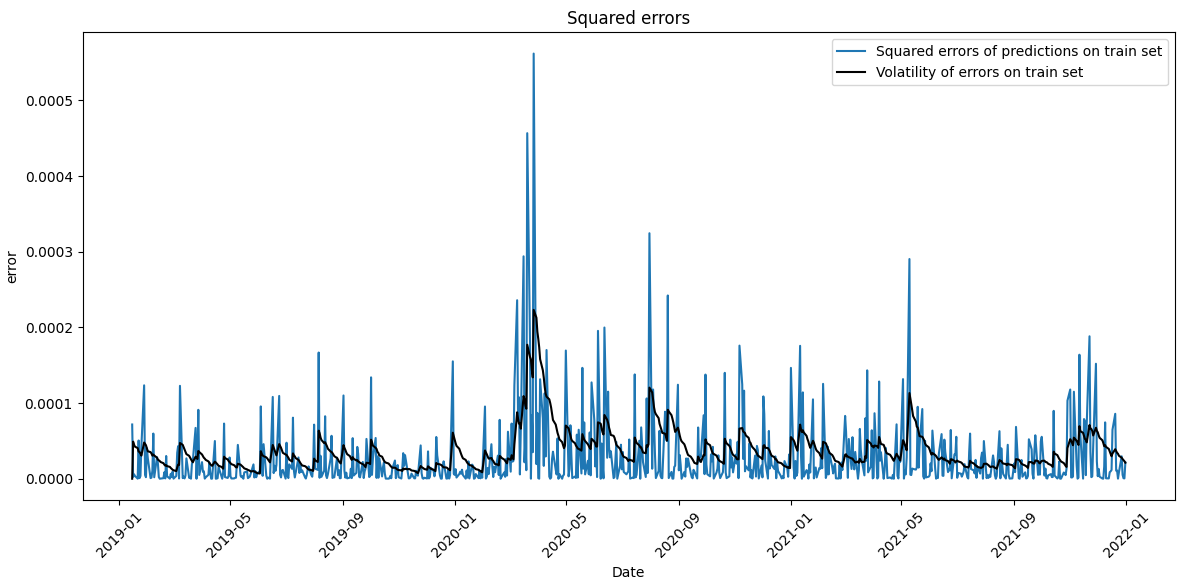
\includegraphics[width=1\textwidth]{Machine_learning_thesis/Images/error volatility.png}
    \caption{Errors volatility.} 
    \label{fig:Errors volatility}
\end{figure}



The actual implementation of the previously described formulations can be summarized by the code snippet: 

\texttt{test\_volatility = ae\_test\_errors.ewm(span=100, adjust=False).std().fillna(0)}. 
For each base model a meta-model is trained to forecast the volatility of prediction errors at the next time step $t+1$. This meta-models gets as input a sliding windows of past volatility values $( v_{t-k}, v_{t-k+1}, \dots, v_t )$ to learn historical patterns, which are then used to predict the volatility of the next time step $v_{t+1}$. The way the predicted volatilities are then converted into dynamic weights can be seen in the code snippet provided below \ref{ensemble prediction implementation}. First the best $k$ volatilities values are selected and normalized, a mask is then applied to the original tensor, assigning an infinite value to the remaining $n-k$ volatilities, effectively excluding them from subsequent calculations. Finally a softmax function is applied to the masked volatility values after scaling them by the a temperature factor. This dynamic weighting mechanism ensures that the ensemble prediction is driven by the models that are expected to perform best in the next time period $t+1$. 
\label{ensemble prediction implementation}
\begin{lstlisting}[language=Python, caption=Ensemble Prediction Implementation]
def predict(self):
    # Parallel execution
    with ThreadPoolExecutor() as executor: 
        results = list(executor.map(self.model_prediction, self.trained_models)) 

        # Combine predictions into a single tensor
        self.test_predictions = torch.stack([item[0] for item in results], dim=1).squeeze()
        self.test_error_predictions = torch.stack([item[1] for item in results], dim=1).squeeze()

        # Filter the k best errors
        best_kerrors, indices = torch.topk(self.test_error_predictions, k=self.k, largest=False, sorted=False)

        # Normalize the errors
        std = best_kerrors.std(dim=1, keepdim=True)
        mean = best_kerrors.mean(dim=1, keepdim=True)
        normalized_errors = (self.test_error_predictions - mean) / std

        # Apply mask
        mask = torch.zeros_like(self.test_error_predictions, dtype=torch.bool)
        mask.scatter_(dim=1, index=indices, value=True)
        normalized_errors[~mask] = float('inf')
    
        # Apply softmax
        weights_df = F.softmax(-normalized_errors * self.temperature, dim=1)

        # Combine predictions
        self.ensemble_preds = (self.test_predictions[self.error_window:] * weights_df).sum(dim=1)
        return self.ensemble_preds
\end{lstlisting}
The library adopts four parameters, which can be adjusted by the user, to govern the ensemble behavior:
\begin{enumerate}
    \item \textbf{k}: The number of top-performing models retained for weighting the predictions
    \item  \textbf{temperature}: Regulates the softmax weighting distribution's sharpness; higher values intensify the focus on the best-performing models, while lower values promote smoother weight distributions
    \item \textbf{meta\_model}: Define which pre-trained meta model type to be used to predict the volatility
    \item \textbf{error\_window}: Defines the number of past values to be considered by the meta-models to predict the next error.
\end{enumerate}

\subsection{Final predictions} 
The final predictions are obtained by summing the linear predictions from the SARIMA model and the non-linear predictions of the residuals from the Arbitrated Dynamic Ensemble. 
\[
\hat{y}_t = \hat{y}_t^{\text{SARIMA}} + \hat{y}_t^{\text{ADE}}
\]
The literature provides strong evidence for this additive aggregation, demonstrating that predicting accuracy is improved by breaking down time series into linear and non-linear components \cite{zhang2003hybrid}.  No additional weighting or scaling is applied afterward since the residuals modeled by the ensemble are already scaled to the same range as the SARIMA predictions. 


\section{Evaluation metrics}
The performance of the models is evaluated using a set of evaluation metrics that capture different aspects of error. 
\subsubsection{Root Mean Squared Error (RMSE)}
It provide an interpretable measure of error on the same scale as the data, computed as:
\[
\text{RMSE} = \sqrt{\frac{1}{n} \sum_{i=1}^{n} (y_i - \hat{y}_i)^2}
\]
but it's highly sensitive to large errors, since errors are squared, and otliers as a consequence will have a larger effect on the RMSE.

\subsubsection{Mean Squared Error}
The Mean Squared Error (MSE) is a measure of the average of the squares of the errors, computed as:
\[
\text{MSE} = \frac{1}{n} \sum_{i=1}^{n} (y_i - \hat{y}_i)^2
\]
Unlike RMSE, the MSE does not take the square root of the error, which means that the values are on the squared scale of the data rather than the same scale as the original values. 

\subsubsection{Mean Absolute Error (MAE)}
It's the average of the absolute errors, computed as.
\[
\text{MAE} = \frac{1}{n} \sum_{i=1}^{n} |y_i - \hat{y}_i|
\]
Unlike RMSE and MSE, which penalize larger errors more heavily due to the squaring of residuals, the Mean Absolute Error treats all errors equally by taking their absolute values, making it less sensible to outliers and more robust to extreme values. MAE is also easier to interpret since it is on the same scale as the data, similar to RMSE. 

\subsubsection{$R^2$ Score}
The $R^2$ score, also known as the \textbf{coefficient of determination}, is a statistical metric that indicates how well the model's predictions fit the actual data. It's defined as  as the percentage of the dependent variable's variation that can be predicted from the independent variables, computed as:
\[
R^2 = 1 - \frac{\sum_{i=1}^{n} (y_i - \hat{y}_i)^2}{\sum_{i=1}^{n} (y_i - \bar{y})^2}
\]
where:
\begin{itemize}
    \item $y_i$ represents the actual values
    \item $\hat{y}_i$ represents the predicted values
    \item $\bar{y}$ is the mean of the actual values.
\end{itemize}
The $R^2$ score ranges from 0 to 1, where:
\begin{itemize}
    \item An $R^2$ of 1 indicates perfect prediction, meaning all the variability in the dependent variable is explained by the model
    \item An $R^2$ of 0 indicates that the model does not explain any of the variability in the data, meaning the model is no better than using the mean of the dependent variable as a prediction
    \item Negative values of $R^2$ can occur when the model performs worse than a horizontal line representing the mean, implying a very poor model fit.
\end{itemize}

\subsubsection{Mean Absolute Percentage Error (MAPE)}
It expresses the prediction accuracy in percentage terms, calculated as the average of the absolute percentage errors between the actual and predicted values:
\[
\text{MAPE} = \frac{1}{n} \sum_{i=1}^{n} \left| \frac{y_i - \hat{y}_i}{y_i} \right| \times 100
\]
MAPE is useful since it provides an error percentage that is easy to interpret, however, it has some notable limitations:
\begin{itemize}
    \item When actual values \( y_i \) are close to zero, MAPE can become extremely large or even undefined, leading to distorted results
    \item MAPE treats positive and negative errors equally, which may not always reflect the relative importance of these errors in certain contexts.
\end{itemize}

\subsubsection{Symmetric Mean Absolute Percentage Error (SMAPE)}
It address some of the issues with MAPE, modifying the formula to make the error symmetric and mitigating the effect of small values in the denominator:
\[
\text{SMAPE} = \frac{1}{n} \sum_{i=1}^{n} \frac{|y_i - \hat{y}_i|}{\frac{|y_i| + |\hat{y}_i|}{2}} \times 100
\]
In the denominator instead of using just \( y_i \), like MAPE, SMAPE uses the average of the absolute values of the actual and predicted values, making it more robust.



